%-----------------------------------------------------------------------------%
% Notizen für die Nachwelt
% von Jens Kallup
%-----------------------------------------------------------------------------%
\documentclass[10pt]{book}
\usepackage{ngerman}
\usepackage{titlesec}
\usepackage{graphicx}
\usepackage{tikz}
\usetikzlibrary{calc}
\usepackage{textpos}
\usepackage{calc}
\usepackage{amsmath, amssymb}
\usetikzlibrary{arrows, decorations.markings}
\usepackage{fancyhdr} 
\usepackage{lastpage}
\usepackage{float} 
\usepackage{pgfplots}
\pgfplotsset{compat=1.9}
\pagestyle{empty}

%%\setmainfont{Arial}
\usepackage{tikz,xcolor,mwe}
\definecolor{cvgreen}{HTML}{92D14F}
\definecolor{cvgray}{HTML}{D8E4BE}
\definecolor{cvtext}{HTML}{000000}
\usetikzlibrary{shadows}

\DeclareFixedFont{\chapternumberfont}{T1}{ppl}{}{}{1.5in}
\titleformat{\chapter}[display]{\Huge\bfseries\sffamily\color{white}}{
%%\thispagestyle{empty}
\begin{tikzpicture}[overlay, remember picture]
        \path let \p1 = (current page.west), \p2 = (current page.east) in
        node[minimum width=\x2-1.5pt, minimum height=5cm,
        rectangle, fill=cyan, anchor=north west, align=left, text width=\x2-\x1] at ($(current page.north west)$) {
        \begin{textblock*}{5in}(\dimexpr\x2-4.0in,\dimexpr0.25\headheight-1in)
          \tikz \node [white,text width=2in, align=right, font=\sffamily] {{\normalsize MATHEMATIK }\\[10pt]
          \raisebox{20pt}{{\large \chaptertitlename}} \raisebox{-12pt}{\chapternumberfont \thechapter}};
        \end{textblock*}};
        \path let \p1 = (current page.west), \p2 = (current page.east) in
              node[minimum width=\x2-\x1, minimum height=-2.8in, rectangle, fill=cyan!50, anchor=south west, align=left, text width=\x2-\x1] at ($(current page.south west)$) {\textcolor{black}{\Large{\thepage . \: \: de.scr.mathematik}}};
\end{tikzpicture}
}{-1.75in}{}[\vspace*{1.25in}]


\newcommand\brectangles{%
\begin{tikzpicture}[overlay, remember picture]
\fill[cyan] 
  (current page.north west) rectangle ( $ (current page.north east) + (0,-7cm) $);
\fill[cyan!30] 
  (current page.south west) rectangle ( $ (current page.south east) + (0,3cm) $);
\end{tikzpicture}%
}

\newcommand\bildzrange{%
\begin{tikzpicture}[overlay, remember picture]
   \node[inner sep=0pt,below right] (image) at ([xshift=-10cm,yshift=-9cm]current page.north east)
  {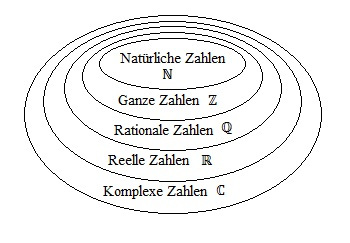
\includegraphics[width=7.5cm,height=4.5cm]{zbereiche.jpg}};
\end{tikzpicture}%
}

\newcommand\legendezbereiche{%
\begin{tabular}{llc}
 $\mathbb{C}$ & = komplexe Zahl    \\
 $\mathbb{I}$ & = irrationale Zahl \\
 $\mathbb{N}$ & = natürliche Zahl  \\
 $\mathbb{Q}$ & = rationale Zahl   \\
 $\mathbb{R}$ & = reelle Zahl      \\
 $\mathbb{Z}$ & = ganze Zahl       
\end{tabular}%
}

\titleformat{name=\chapter,numberless}[display]
  {\Huge\bfseries\sffamily\color{white}}
  {\thispagestyle{empty}\brectangles} 
  {-1in}
  {\parbox[b]{.65\linewidth}{1}}
  [\vspace*{1in}]

\begin{document}
\title{Mathe Notizen}
\author{Jens Kallup}
\date{\today}

\begin{tikzpicture}[remember picture,overlay]
    % green bar
    \fill[cvgreen] (current page.north west) rectangle ([xshift=5cm]current page.south west);
    % gray bar
    \fill[cvgray] ([yshift=-5cm]current page.north west) rectangle ([yshift=-10cm]current page.north east);
    % title and date
    \node[cvtext,right] at ([yshift=-7cm]current page.north west) {\Huge\bfseries Mathe-Notizen f\"ur Selbstudium};
    \node[cvtext,right] at ([yshift=-8cm]current page.north west) {\Huge 1. Auflage};
    \node[cvtext,above left] at ([xshift=-1cm,yshift=-9.5cm]current page.north east) {\Huge\bfseries vom \today };
    % cover photo
    \node[inner sep=0pt,below right] (image) at ([xshift=5cm,yshift=-10cm]current page.north west)
    {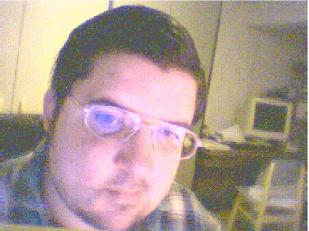
\includegraphics[width=11cm,height=9cm]{me.jpg}};
    % name and address
    \node[fill=white,drop shadow,align=center,text width=6.4cm,inner sep=0.3cm,below] (name) at (image.south)
        {\LARGE Jens Kallup};
    \node[text width=15cm,inner sep=0.3cm,below right] at (name.south west) {\Large\obeylines%
        Langensalzer Str. 30
        99817 Eisenach
        Tel.: 03691 /
        E-Mail: jkallup@web.de
    };
    % attachments
    \node[white,text width=5cm,inner sep=0.3cm,above right] at ([yshift=1cm]current page.south west) {\large\obeylines%
        \textbf{Inhalt:}
        Eigene Gedanken
        zu: de.sci.mathematik
    };
\end{tikzpicture}


\tableofcontents

\chapter{Vorwort}
mit diesen Posting will ich versuchen, eine Zusammenfassung
dessen zu geben, was hier seit Monaten Diskutiert wird.
Falls was falsch sein sollte, bitte Feedback geben.
Kann auch passieren das ich aus versehen eine falsche Taste
beim schreiben drücke, und der Inhalt fehlt, ich bemühe mich
durchgängig zu schreiben und im Zusammenhang zu posten.
Ok, let's go...

\chapter{Grundlagen}
\section{Zeichen und Symbole}

\begin{minipage}{0.5\textwidth}
  \begin{tabular}{lcr}
    \legendezbereiche & \\ \\ \bildzrange
  \end{tabular}
\end{minipage}

\chapter{Zahlen und Zahlenbereiche}

\section{Nat"urliche Zahlen}
\begin{itemize}
  \item[1.] Nat"urliche Zahlen $N$ sind \textbf{positive} Zahlen, die durch 0
            bis 9 symbolisiert dargestellt werden.
            Nat"urliche Zahlen k"onnen gepaart werden, indem man an den Zahlen 1 bis 9
            weitere natürliche Zahlen anf"ugt (zum Bsp.: 12, 34, 22).
            Bei der Aufstellung der nat"urlichen Zahlen ist wie in der mathelogie
            "ublich eine einheitliche Form einzuhalten.
            So kann/darf man bei einer Definition nicht einfach: 12, 1 33
            schreiben !!!
            Es ist zwar keine feste Regel dafür manifestiert, aber der "Ubersichtlichkeit
            ist eine gewisse Disziplin der Ordnung nicht falsch. \\

            Die Menge der nat"urlichen \textbf{positiven} Zahlen werden wie folgt
            definiert: \\
            $N = \{ 0;1;2;3; \ldots \}$ \\

            Nat"urliche Zahlen sind nur innerhalb eines mehr oder weniger
            gro"sen Bereichs abz"ahlbar, da sie unendlich sind. Jede nat"urliche Zahl
            \textbf{n} hat immer einen unmittelbaren Nachfolger \textbf{n + 1} hat.
  \item[2.] ganze Zahlen $Z$ erweitern die nat"urlichen Zahlen $N$.
  \item[3.] rationale Zahlen $Q$ entsprechen dem Verhältnis zweier ganzer Zahlen $Z$
            (siehe Bruchrechnen).
  \item[3.1.] gebrochene Zahlen $Q+$ oder $Q*$ sind eine Erweiterung der nat"urlichen
              Zahlen $N$, die gestattet, uneingeschränkt zu dividieren.
              Dazu werden nat"urliche Zahlen um den \textbf{negativen} Zahlenbereich von
              $N$ sowie um Br"uche (rationale Zahlen $Q$) erg"anzt.

  \item[3.2.] Addition und Maltiplikation k"onnen als ''abgeschlossene Operationen'' betrachtet werden.
              Die Summe zweier nat"urlicher Zahlen ergibt immer eine weitere nat"urliche Zahl:
              \\
              $3 + 5 = 8 \:\:\:\:\:\:\: | \:\: 3 \in \mathbb{N}; \: 5 \in \mathbb{N}; \: 8 \in \mathbb{N} \\
              3 \: * 5 = 15 $
              \\
              \\
              \textbf{Minus und Division} gelten als ''nicht abgeschlossene Operationen''.
              Die Differenz zweier nat"urlicher Zahlen muss nicht immer eine
              nat"urliche ergeben:

             $3 - 5 = \: -2 \: \: \: | \: 3 \in \mathbb{N}; \: 5 \in \mathbb{N} \: -2 \notin \mathbb{N} \\
              3 \: : 5 \: = \: 0,6 \: \: | \: 3 \in \mathbb{N}; \: 5 \in \mathbb{N} \:\: 0.6 \notin \mathbb{N}$
\\
\\
\textbf{Bonus:}\\
\marginpar[\textbf{www.lernhelfer.de}]{\textbf{www.lernhelfer.de}}
        Im Internet habe ich ein etwas verungl"ucktes Beispiel
        zu unendliche N gefunden, das ich hier vorstellen, aber auch
        Kommentieren will.\\
\\
        - man denke sich ein kosmisches Hotel mit unendlich vielen
          Zimmern vor.\\
        - das Hotel ist *voll* belegt.\\
        - Nun kommt noch ein Gast.\\
\\
        Frage: Kann er in einen voll belegten Hotel noch untergebracht
               werden?
        Antwort: = JA! \\

        - da es unendlich viele Zimmer gibt, rückt jeder Gast nur ein
          Zimmer weiter und das erste wird frei.\\
        - nach dem selben Prinzip k"onnen nat"urlich auch weitere 10 G"aste
          untergebracht werden.

        Kommentar von mir dazu:\\
        Der Sichtwinkel ist hierbei wichtig!
        Logisch ist es, wenn man von einen *vollen* Hotel spricht, das
        alle Betten belegt sind.
        Da aber der Begriff ''unendlich'', kein Ende oder *voll* definiert
        ist, k"o"nnen auch ''unendlich'' viele Betten/Zimmer bezogen werden.

        Anders ausgedr"uckt kann  die Zahl unendlich, kann an die Zahl
        unendlich angekn"upft werden, um wieder eine Menge von unendlich
        und nicht abz"ahlbaren Zahlen zu bekommen.

  \item[4.] reelle Zahlen $\mathbb{R}$ erweitern den Zahlenbereich der
            rationalen Zahlen $\mathbb{Q}$ sowie den Zehlenbereich der Br"uche.
  \item[4.1.] reelle Zahlen umfassen auch den Zahlenbereich der
              irrationalen Zahlen $\mathbb{I}$ .

  \item[5.] komplexe Zahlen $\mathbb{C}$ erweitern den Zahlenbereich des reellen
            Zahlenbereichs.\\
            Beispiel solcher Zahlen sind: $i, 7 + 3i, 3 - 4i$\\

    Mit fortschreitender Erlangung von neuen Kenntnissen (z. Bsp. auch gepr"agt
    von der Nutzung elektronischer Einheiten; womit ich
    die Einf"uhrung des mathematische Bin"arsystems - $n^2$ andeuten will), wurde man
    dadurch motiviert, komplexe Zahlen einzuf"uhren.\\
    Man erkannte, das Gleichungen wie $x^2 = -1$ nicht l"osbar sind.
    Da es nun aber auch die Zahl -1 (gesprochen: minus eins) in der
    Zahlentheorie gibt, wurde eine \textbf{imaginäre Einheit} eingef"uhrt, die mit \textbf{i}
    - als Definition: \textbf{ $ i^2 = -1 $ }  manifestiert wurde.
    Mit komplexen Zahlen wurde somit das Problem behoben.
\end{itemize}
\subsection{Beispiel aus de.sci.mathematik}

Gegeben ist folgende Gleichung: \\ \\
$\sqrt[n]{(e^{(i \phi)}) = e^{i * (\frac{\phi}{n} + k * 2 * \frac{\pi}{n})} } $ mit  $ k = 0, 1, 2,..., n-1. $ \\

Hier die einfache Herleitung: \\
F"ur n = 2 und k = 0 aus der Gleichung: \\
\\
e entspricht der Eulerzahl 1 \\
i entspricht der imaginären Zahl: \: $ i^2 = -1 $ \\
dann ergibt sich aus e und i: \: $ 1^2 = -1 $ \\
$ \phi $ entsprich 1 * phi \\
$ \frac{\pi}{2} $ entsprich die H"alfte der Kreiszahl $\pi $: $ \frac{3.14}{2} = 1.57 $ \\
\\
1. $ \sqrt[2]{1^{-1 * \phi} = 1^{-1 * (\frac{\phi}{2} + 0 * 2 * \frac{\pi}{2})}} $ \\
2. $ \sqrt[2]{1^{-1 * \phi} = 1^{-1 * (\frac{\phi}{2} + 0 * 2 * 1.57)}} $ \\
3. $ \sqrt[2]{1^{-\phi} = \frac{1 * 2}{1} * \frac{\phi}{2}}  \: \: \: | \: \: 2 \: und \: 2 \: k"urzt \: sich \: weg. \: (\phi = 1)$\\
4. $ \sqrt[2]{1^{-1} = 1 * 1} $ \\
5. $ \sqrt[2]{1 = 1} = \sqrt[2]{1} = \sqrt[2]{1} $ \\
6. $ 1 = 1 $

\chapter{Mengen}
Mengen k"onnen auf zwei verschiedene weisen dargestellt werden:
\begin{itemize}
  \item[1.]   \textbf{aufz"ahlende Schreibweise:}\\
  Alle Elemente einer Menge in geschweifter Klammer:
  $M = \{ 1;2;3 \}$ \\ \\
  Wenn in einer Menge ein l"angeres Intervall existiert,
  kann man sich durch Schreibweise \ldots bedienen.
  Diese Schreibweise kennzeichnet Elemente, die in der
  Menge *M* vorkommen k"onnen, jedoch aus Platzgründen
  nicht mit aufgeschrieben werden - man k"onnte es auch
  als Platzhalter verstehen. \\
  Und hier noch die Schreibweise: 
  $M = \{ 1;2;3; \ldots ;10;11 \}$
  \item[2.] \textbf{die beschreibende Schreibweise:} \\
  Mit dieser Schreibweise wird versucht, Elemente einer
  Menge mit mathematischen Aussagen zu beschreiben. Erf"ullt
  ein Element eine Aussage, so ist dieses Element der Menge: \\
  $M = \{ \: p \: | \: '' p \: ist \: eine \: Primzahl '' \: \}$ \\
  \\
  Sei Menge M eine mathematisch beschreibende Aussage:\\
  $M = \{z \in N \}$ \\
  \\
  dann spricht man von einer Menge M, in der ''z Element von N ist''. \\
  Wenn gilt: $M = \{z \le 17\}$\\
  \\
  dann spricht man von einer Menge, in der nur das Element z
  kleiner gleich 17 enthalten sein darf/ (oder alle Elemente
  von z kleiner gleich 17 sind). \\
\end{itemize}
Mengendiagramme sind Diagramme, die Elemente in einer
geschlossener Umgebung enthalten.



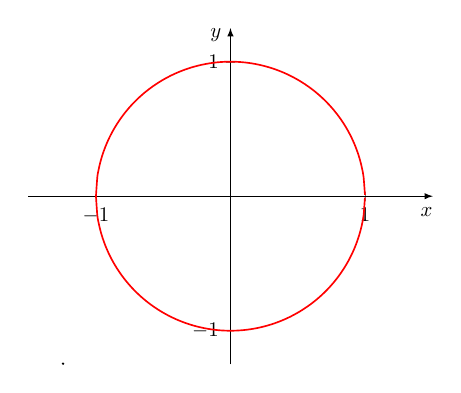
\begin{tikzpicture}[scale=0.75]
\begin{axis}[
  xmin = -1.25, xmax = 1.25,
  ymin = -1.25, ymax = 1.25,
  samples = 200,
  axis lines = middle,
  axis equal,
  axis line style = {-latex},
  xlabel = {$x$},
  xtick={-1,...,1},
  ylabel = {$y$},
  ytick={-1,...,1},
  xlabel style={
    yshift=-.5*\pgfkeysvalueof{/pgfplots/major tick length},
    anchor=north east,
    inner xsep=0pt
  },
  ylabel={\normalsize $y$},
  ylabel style={
    xshift=-.2*\pgfkeysvalueof{/pgfplots/major tick length},
    anchor=north east,
    inner ysep=0pt
  },
  every axis plot/.append style={
    domain = -1:1,
    smooth,
    thick,
    no markers
  }
]
  \addplot[red]{(1 - x^2)^0.5};
  \addplot[red]{-(1 - x^2)^0.5};
  \draw[thick](1,0) -- (0,1) node[near start, below]{$s$};
\end{axis}
\end{tikzpicture}

\end{document}
